\documentclass{article}

\usepackage[dvipsnames,svgnames,x11names,table]{xcolor}
\usepackage{fancyhdr}
\usepackage{extramarks}
\usepackage{amsmath}
\usepackage{amsthm}
\usepackage{amsfonts}
\usepackage{tikz}
\usepackage[plain]{algorithm}
\usepackage{algpseudocode}
\usepackage{enumerate}
\usepackage{amssymb}
\usepackage{unicode-math}
\usepackage{multicol}
\usepackage{booktabs}

\usepackage{graphicx}
\usepackage{adjustbox}
\usepackage{varwidth,pst-tree,realscripts}
\usepackage{rotating}
\usepackage{bidi}

\usepackage{forest}
\usepackage{tabularx}

\psset{showbbox=false,treemode=D,linewidth=0.8pt,treesep=0.25cm,levelsep=1cm}
\newcommand{\LFTw}[2]{%
\TR[ref=#1]{\psframebox[linestyle=none,framesep=4pt]{%
\begin{varwidth}{15ex}\center #2\end{varwidth}}}}
\newcommand{\LFTr}[2]{\TR[ref=#1]{\psframebox[linestyle=none,framesep=4pt]{#2}}}

\usetikzlibrary{automata,positioning,arrows,shapes.geometric,arrows.meta}

%
% Basic Document Settings
%

\topmargin=-0.45in
\evensidemargin=0in
\oddsidemargin=0in
\textwidth=6.5in
\textheight=9.0in
\headsep=0.25in
\setmathfont{XITS Math}
\setmathfont[version=setB,StylisticSet=1]{XITS Math}

\linespread{1.5}

\pagestyle{fancy}
\lhead{\hmwkAuthorName}
\chead{\tiny\hmwkClass\ (\hmwkClassInstructor\ \hmwkClassTime): \hmwkTitle}
\rhead{\firstxmark}
\lfoot{\lastxmark}
\cfoot{\thepage}

\renewcommand\headrulewidth{0.4pt}
\renewcommand\footrulewidth{0.4pt}

\setlength\parindent{0pt}

%
% Create Problem Sections
%

\newcommand{\enterProblemHeader}[1]{
    \nobreak\extramarks{}{Problem \arabic{#1} continued on next page\ldots}\nobreak{}
    \nobreak\extramarks{Problem \arabic{#1} (continued)}{Problem \arabic{#1} continued on next page\ldots}\nobreak{}
}

\newcommand{\exitProblemHeader}[1]{
    \nobreak\extramarks{Problem \arabic{#1} (continued)}{Problem \arabic{#1} continued on next page\ldots}\nobreak{}
    \stepcounter{#1}
    \nobreak\extramarks{Problem \arabic{#1}}{}\nobreak{}
}

\setcounter{secnumdepth}{0}
\newcounter{partCounter}
\newcounter{homeworkProblemCounter}
\setcounter{homeworkProblemCounter}{1}
\nobreak\extramarks{Problem \arabic{homeworkProblemCounter}}{}\nobreak{}

%
% Homework Problem Environment
%
% This environment takes an optional argument. When given, it will adjust the
% problem counter. This is useful for when the problems given for your
% assignment aren't sequential. See the last 3 problems of this template for an
% example.
%
\newenvironment{homeworkProblem}[1][-1]{
    \ifnum#1>0
        \setcounter{homeworkProblemCounter}{#1}
    \fi
    \section{Problem \arabic{homeworkProblemCounter}}
    \setcounter{partCounter}{1}
    \enterProblemHeader{homeworkProblemCounter}
}{
    \exitProblemHeader{homeworkProblemCounter}
}

%
% Homework Details
%   - Title
%   - Due date
%   - Class
%   - Section/Time
%   - Instructor
%   - Author
%

\newcommand{\hmwkTitle}{Assignment\ \#2}
\newcommand{\hmwkDueDate}{27 September 2023}
\newcommand{\hmwkClass}{CSE 486 – Introduction to Artificial Intelligence}
\newcommand{\hmwkClassTime}{Section A}
\newcommand{\hmwkClassInstructor}{Dr Khodakhast Bibak}
\newcommand{\hmwkAuthorName}{\textbf{Emil Sayahi}}

%
% Title Page
%

\title{
    \vspace{2in}
    \textmd{\textbf{\hmwkClass:\ \hmwkTitle}}\\
    \normalsize\vspace{0.1in}\small{Due\ on\ \hmwkDueDate\ at 11:59pm}\\
    \vspace{0.1in}\large{\textit{\hmwkClassInstructor\ \hmwkClassTime}}
    \vspace{3in}
}

\author{\hmwkAuthorName}
\date{}

\renewcommand{\part}[1]{\textbf{\large Part \Alph{partCounter}}\stepcounter{partCounter}\\}

%
% Various Helper Commands
%

% Useful for algorithms
\newcommand{\alg}[1]{\textsc{\bfseries \footnotesize #1}}

% For derivatives
\newcommand{\deriv}[1]{\frac{\mathrm{d}}{\mathrm{d}x} (#1)}

% For partial derivatives
\newcommand{\pderiv}[2]{\frac{\partial}{\partial #1} (#2)}

% Integral dx
\newcommand{\dx}{\mathrm{d}x}

% Alias for the Solution section header
\newcommand{\solution}{\textbf{\large Solution}}

% Probability commands: Expectation, Variance, Covariance, Bias
\newcommand{\E}{\mathrm{E}}
\newcommand{\Var}{\mathrm{Var}}
\newcommand{\Cov}{\mathrm{Cov}}
\newcommand{\Bias}{\mathrm{Bias}}

\begin{document}

\maketitle

\pagebreak

% Problem 1
\begin{homeworkProblem}
    \textbf{(8 points)} Suppose we want to construct three new airports in a given country. The objective is to minimize the distance from each city to its nearest airport. Describe the gradient descent and explain how this technique can help us to solve this problem. Write your solution mathematically as we
    discussed in class.\\

    \solution\\
    TODO
\end{homeworkProblem}

\pagebreak

% Problem 2
\begin{homeworkProblem}
    \textbf{(0 points)} Optional.
\end{homeworkProblem}

\pagebreak

% Problem 3
\begin{homeworkProblem}
    \textbf{(0 points)} Optional.
\end{homeworkProblem}

\pagebreak

% Problem 4
\begin{homeworkProblem}
    \textbf{(4 points)}

    \part
    \textbf{(2 points)} Give a set of broad conditions under which $A^{*}$ search reduces to BFS.\\
    
    \solution\\
    TODO\\

    \part
    \textbf{(2 points)} Does $A^{*}$ always return an optimal solution? Explain.\\

    \solution\\
    TODO

\end{homeworkProblem}

\pagebreak

% Problem 5
\begin{homeworkProblem}
    \textbf{(6 points)}

    \part
    \textbf{(3 points)} When would DFS be a better choice than $A^{*}$ search?\\

    \solution\\
    TODO\\

    \part
    \textbf{(3 points)} Which path will $A^{*}$ return for the following search problem?\\
    \begin{figure}[ht]
        \centering
        \begin{minipage}{0.4\textwidth}
            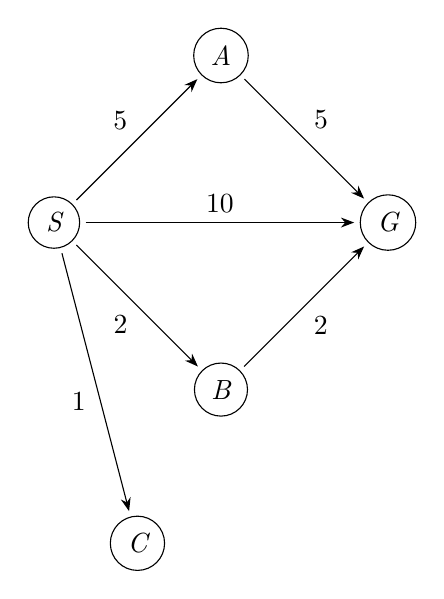
\begin{tikzpicture}[shorten >=4pt,node distance=3cm,on grid,auto,font=\itshape]
                \node[draw,circle] (s)   {S};
                \node[draw,circle,above right of=s] (a)   {A};
                \node[draw,circle,below right of=s] (b)   {B};
                \node[draw,circle,below=of $(s.north)!0.5!(b.north)$] (c)   {C};
                \node[draw,circle,below right of=a] (g)   {G};
                \path[-Stealth,shorten >= 2pt, shorten <= 2pt,font=\upshape]
                    (s)
                        edge node {5} (a)
                        edge node[below left] {2} (b)
                        edge node[below left] {1} (c)
                        edge node {10} (g)
                    (a)
                        edge node {5} (g) 
                    (b)
                        edge node[below right] {2} (g);
            \end{tikzpicture}
        \end{minipage}
        \hfill
        \begin{minipage}{0.4\textwidth}
            \begin{tabular}{|cc|}
                \hline
                Node & $h$\\
                \hline
                $S$ & $4$\\
                $A$ & $3$\\
                $B$ & $2$\\
                $C$ & $100$\\
                $G$ & $0$\\
                \hline
            \end{tabular}
        \end{minipage}
    \end{figure}\\

    \solution\\
    TODO
    
\end{homeworkProblem}

\pagebreak

% Problem 6
\begin{homeworkProblem}
    \textbf{(6 points)}\\

    \part
    \textbf{(4 points)} Consider the zero-sum game tree shown below. Triangles that point up, such as at the top
    node (root), represent choices for the maximizing player; triangles that point down represent
    choices for the minimizing player. Assuming both players act optimally, fill in the minimax value of
    each node.
    \begin{figure}[ht]
        \centering
        \begin{tikzpicture}[square/.style={regular polygon,regular polygon sides=4},scale=1.5,font=\footnotesize]
            \tikzstyle{solid node}=[circle,draw,inner sep=1.5,fill=black]
            \tikzstyle{hollow node}=[circle,draw,inner sep=1.5]
            \tikzstyle{level 1}=[level distance=15mm,sibling distance=3.5cm]
            \tikzstyle{level 2}=[level distance=15mm,sibling distance=1.5cm]
            \tikzstyle{level 3}=[level distance=15mm,sibling distance=1cm]
            \node(0)[isosceles triangle,isosceles triangle apex angle=60,draw,rotate=90]{}
              child{node[isosceles triangle,isosceles triangle apex angle=60,draw,rotate=270]{}
                child{node[square,draw]{$10$} edge from parent node[left]{}}
                child{node[square,draw]{$8$} edge from parent node[left]{}}
                child{node[square,draw]{$3$} edge from parent node[right]{}}
                edge from parent node[left,xshift=-5]{}
              }
              child{node[isosceles triangle,isosceles triangle apex angle=60,draw,rotate=270]{}
                child{node[square,draw]{$2$} edge from parent node[left]{}}
                child{node[square,draw]{$15$} edge from parent node[left]{}}
                child{node[square,draw]{$7$} edge from parent node[right]{}}
                edge from parent node[left,xshift=-5]{}
              }
              child{node[isosceles triangle,isosceles triangle apex angle=60,draw,rotate=270]{}
                child{node[square,draw]{$6$} edge from parent node[left]{}}
                child{node[square,draw]{$5$} edge from parent node[right]{}}
                child{node[square,draw]{$4$} edge from parent node[right]{}}
                edge from parent node[right,xshift=5]{}
              };
          \end{tikzpicture}
    \end{figure}
    \\

    \solution\\
    \begin{figure}[ht]
        \centering
        \begin{tikzpicture}[square/.style={regular polygon,regular polygon sides=4},scale=1.5,font=\footnotesize]
            \tikzstyle{solid node}=[circle,draw,inner sep=1.5,fill=black]
            \tikzstyle{hollow node}=[circle,draw,inner sep=1.5]
            \tikzstyle{level 1}=[level distance=15mm,sibling distance=3.5cm]
            \tikzstyle{level 2}=[level distance=15mm,sibling distance=1.5cm]
            \tikzstyle{level 3}=[level distance=15mm,sibling distance=1cm]
            \node(0)[isosceles triangle,isosceles triangle apex angle=60,draw,rotate=90]{\rotatebox{270}{$4$}}
              child{node[isosceles triangle,isosceles triangle apex angle=60,draw,rotate=270]{\rotatebox{90}{$3$}}
                child{node[square,draw]{$10$} edge from parent node[left]{}}
                child{node[square,draw]{$8$} edge from parent node[left]{}}
                child{node[square,draw]{$3$} edge from parent node[right]{}}
                edge from parent node[left,xshift=-5]{}
              }
              child{node[isosceles triangle,isosceles triangle apex angle=60,draw,rotate=270]{\rotatebox{90}{$2$}}
                child{node[square,draw]{$2$} edge from parent node[left]{}}
                child{node[square,draw]{$15$} edge from parent node[left]{}}
                child{node[square,draw]{$7$} edge from parent node[right]{}}
                edge from parent node[left,xshift=-5]{}
              }
              child{node[isosceles triangle,isosceles triangle apex angle=60,draw,rotate=270]{\rotatebox{90}{$4$}}
                child{node[square,draw]{$6$} edge from parent node[left]{}}
                child{node[square,draw]{$5$} edge from parent node[right]{}}
                child{node[square,draw]{$4$} edge from parent node[right]{}}
                edge from parent node[right,xshift=5]{}
              };
          \end{tikzpicture}
    \end{figure}\\

    \part
    \textbf{(2 points)} Which nodes can be pruned from the game tree above through alpha-beta pruning? If no
    nodes can be pruned, explain why not. Assume the search goes from left to right; when choosing
    which child to visit first, choose the left-most unvisited child.\\

    \solution\\
    TODO
    
\end{homeworkProblem}

\pagebreak

% Problem 7
\begin{homeworkProblem}
    \textbf{(6 points)}\\

    \part
    \textbf{(4 points)} Again, consider the same zero-sum game tree, except that now, instead of a minimizing player,
    we have a chance node that will select one of the three values uniformly at random. Fill in the
    expectiminimax value of each node. The game tree is redrawn below for your convenience.
    \begin{figure}[ht]
        \centering
        \begin{tikzpicture}[square/.style={regular polygon,regular polygon sides=4},scale=1.5,font=\footnotesize]
            \tikzstyle{solid node}=[circle,draw,inner sep=1.5,fill=black]
            \tikzstyle{hollow node}=[circle,draw,inner sep=1.5]
            \tikzstyle{level 1}=[level distance=15mm,sibling distance=3.5cm]
            \tikzstyle{level 2}=[level distance=15mm,sibling distance=1.5cm]
            \tikzstyle{level 3}=[level distance=15mm,sibling distance=1cm]
            \node(0)[isosceles triangle,isosceles triangle apex angle=60,draw,rotate=90]{}
              child{node[circle,draw]{}
                child{node[square,draw]{$10$} edge from parent node[left]{}}
                child{node[square,draw]{$8$} edge from parent node[left]{}}
                child{node[square,draw]{$3$} edge from parent node[right]{}}
                edge from parent node[left,xshift=-5]{}
              }
              child{node[circle,draw]{}
                child{node[square,draw]{$2$} edge from parent node[left]{}}
                child{node[square,draw]{$15$} edge from parent node[left]{}}
                child{node[square,draw]{$7$} edge from parent node[right]{}}
                edge from parent node[left,xshift=-5]{}
              }
              child{node[circle,draw]{}
                child{node[square,draw]{$6$} edge from parent node[left]{}}
                child{node[square,draw]{$5$} edge from parent node[right]{}}
                child{node[square,draw]{$4$} edge from parent node[right]{}}
                edge from parent node[right,xshift=5]{}
              };
          \end{tikzpicture}
    \end{figure}
    \\

    \solution\\
    \begin{figure}[ht]
        \centering
        \begin{tikzpicture}[square/.style={regular polygon,regular polygon sides=4},scale=1.5,font=\footnotesize]
            \tikzstyle{solid node}=[circle,draw,inner sep=1.5,fill=black]
            \tikzstyle{hollow node}=[circle,draw,inner sep=1.5]
            \tikzstyle{level 1}=[level distance=15mm,sibling distance=3.5cm]
            \tikzstyle{level 2}=[level distance=15mm,sibling distance=1.5cm]
            \tikzstyle{level 3}=[level distance=15mm,sibling distance=1cm]
            \node(0)[isosceles triangle,isosceles triangle apex angle=60,draw,rotate=90]{\rotatebox{270}{$8$}}
              child{node[circle,draw]{$7$}
                child{node[square,draw]{$10$} edge from parent node[left]{}}
                child{node[square,draw]{$8$} edge from parent node[left]{}}
                child{node[square,draw]{$3$} edge from parent node[right]{}}
                edge from parent node[left,xshift=-5]{}
              }
              child{node[circle,draw]{$8$}
                child{node[square,draw]{$2$} edge from parent node[left]{}}
                child{node[square,draw]{$15$} edge from parent node[left]{}}
                child{node[square,draw]{$7$} edge from parent node[right]{}}
                edge from parent node[left,xshift=-5]{}
              }
              child{node[circle,draw]{$5$}
                child{node[square,draw]{$6$} edge from parent node[left]{}}
                child{node[square,draw]{$5$} edge from parent node[right]{}}
                child{node[square,draw]{$4$} edge from parent node[right]{}}
                edge from parent node[right,xshift=5]{}
              };
          \end{tikzpicture}
    \end{figure}\\

    \part
    \textbf{(2 points)} Which nodes can be pruned from the game tree above through alpha-beta pruning? If no
    nodes can be pruned, explain why not.\\

    \solution\\
    TODO
    
\end{homeworkProblem}

\end{document}